%% Shared body for main.tex (anonymous) and main_named.tex.
%% All numbers come from generated/macros.tex and generated/table_*.tex (scripts/make_tables.py).
%%
%% STATUS (2026-11-14).  Revised for review v5: 9-page version (TRUST 2027 limit, appendices count);
%%   everything beyond the limit lives in supplement.tex (compiled separately as main_supplement.tex).
%%   Headline = Qwen2.5-7B (Q4_K_M), three seeds (L macros, counts are means per seed); 1.5B = N macros;
%%   offline = O macros.  Intervals are paired cluster bootstraps over the 50 test items.
%%   Compile with XeLaTeX.

\begin{abstract}
Public-service retrieval-augmented generation (RAG) must ground its answers, serve every language fairly, and abstain when the evidence is weak, yet these properties are usually studied separately. We present SL-PubServ-QA, a parallel benchmark of 62 items (\Lnq{} queries in English, Sinhala, Tamil, and code-switched Sinhala--English, every non-English query reviewed by a native speaker) over text quoted from seven Sri Lankan government agencies; an audit record that lets any answer/defer/refuse rule be measured per language; and a cost analysis that prices each rule by the unsafe deliveries (wrong answers, or any answer to an unanswerable query) it removes against the correct answers it withholds. TriSafe-RAG, our reference rule, gates each draft on a five-signal confidence score, per-sentence NLI grounding, and citation coverage. On the \Lntest-query test split with Qwen2.5-7B-Instruct, averaged over three generation seeds, the vanilla pipeline delivers \LBoneUnsafe{} unsafe answers, \LBoneUnsafesi{} of them in Sinhala and \LBoneUnsafeta{} in Tamil. Dev-tuned TriSafe-RAG cuts these to \LTunUnsafe{} but delivers \LTunLostVsBone{} fewer correct answers, lowering decision accuracy from \LBoneDec{} to \LTunDec; it beats the vanilla pipeline only if one unsafe delivery costs more than \LTunBreakEven{} withheld correct answers (95\% CI \LTunBreakEvenCI), and a retrieval-only abstention rule beats it above a cost of \LCrossTunBthree. Two simpler rules dominate it. A filter for replies that contain only citation markers, found by adjudicating every delivered test answer of one seed (\LAdjEmpty{} of \LAdjN) and confirmed on the development split, cuts unsafe deliveries to \LBemptyUnsafe{} at a cost of \LBemptyLostVsBone{} correct answers; adding TriSafe-RAG to that filter leaves \LTemptyUnsafe{} but pays off only above a cost of \LTemptyBreakEvenEmpty. Above a cost of about \LEsixBreakEvenEmpty, translating the query before retrieval has the lowest loss of all. The five-signal confidence is not better calibrated than retrieval similarity (ECE \LTunEce{} versus \LBoneEce). The evidence rests on a small corpus, a 4-bit 7B model, and translations reviewed by one author who is a native speaker. Code, benchmark, cached outputs, adjudication labels, and the scripts that regenerate every number are released.
\end{abstract}

\begin{CCSXML}
<ccs2012>
   <concept>
       <concept_id>10010147.10010178.10010179.10010182</concept_id>
       <concept_desc>Computing methodologies~Natural language generation</concept_desc>
       <concept_significance>500</concept_significance>
       </concept>
   <concept>
       <concept_id>10002951.10003317.10003347.10003352</concept_id>
       <concept_desc>Information systems~Question answering</concept_desc>
       <concept_significance>300</concept_significance>
       </concept>
   <concept>
       <concept_id>10003456.10003462.10003588</concept_id>
       <concept_desc>Social and professional topics~Government technology policy</concept_desc>
       <concept_significance>300</concept_significance>
       </concept>
 </ccs2012>
\end{CCSXML}

\ccsdesc[500]{Computing methodologies~Natural language generation}
\ccsdesc[300]{Information systems~Question answering}
\ccsdesc[300]{Social and professional topics~Government technology policy}

\keywords{trustworthy AI, multilingual NLP, retrieval-augmented generation, selective abstention, fairness, auditability, calibration, public-service AI}

\maketitle

\section{Introduction}
A citizen asks a public-service chatbot in Sinhala what the one-day passport service costs. The system retrieves three English passages, generates a fluent Sinhala reply, and gets the fee wrong. Nothing in the pipeline noticed: the retriever returned its top hits, the generator produced text, and the exchange was logged as a success.

The failure is common. Multilingual RAG systems prefer English passages even for low-resource queries~\cite{park2025langpref}, inherit the biases of their retrievers~\cite{wu2024ragfair}, and contradict the passages they cite~\cite{niu2024ragtruth}. Each of these problems has its own benchmark and its own fix, and the fixes do not compose: a grounding check does not stop a system from under-serving Tamil users, a fairness audit does not stop a confident unsupported answer, and an abstention threshold does not say whether caution was equal across languages. In a public-service deployment the cost of each error is borne by a citizen.

This paper asks a narrower question than ``how to make such a system safe'': how to \emph{measure}, per language and before deployment, what a given answer/defer/refuse rule does, and what a wrong answer has to cost before the rule is worth its coverage. We make four contributions.
\begin{enumerate}
  \item \textbf{A parallel public-service benchmark.} SL-PubServ-QA has 62 items asked in English, Sinhala, Tamil, and (for 22 items) romanised code-switched Sinhala--English (\Lnq{} queries, 10 unanswerable items), over \Lndocs{} documents quoted from seven Sri Lankan agencies, with every non-English query reviewed by a native speaker and an item-level development/test split (Sec.~\ref{sec:benchmark}).
  \item \textbf{An audit record and a reference rule.} One record per decision carries the retrieval scores, per-sentence grounding, citation coverage, confidence, decision, and reason, so any rule can be audited per language. TriSafe-RAG is our reference rule: a five-signal confidence with a three-way policy (Sec.~\ref{sec:method}).
  \item \textbf{A cost analysis.} We separate unsafe deliveries from withheld correct answers and report, for every rule and pair of rules, the break-even cost of one unsafe delivery (Sec.~\ref{sec:cost}). This is the number a deployment needs and decision accuracy hides.
  \item \textbf{A result that goes against our own rule.} On a 7B generator the reference rule is dominated by a content filter found through adjudication and, at high cost, by translating the query; its confidence score is not better calibrated than retrieval similarity; and a self-consistency gate that looked free on one seed tunes to inaction on three (Sec.~\ref{sec:results}). Every number is regenerated from released per-query records by one script.
\end{enumerate}

\section{Related Work}\label{sec:related}
\textbf{Multilingual RAG.} Cross-lingual retrievers such as multilingual-e5~\cite{wang2024me5} have closed much of the retrieval gap, but instruction-tuned generators still prefer English passages and answers when the query is in another language~\cite{park2025langpref,yang2024langbias}, so a system can be multilingual at the input and monolingual in its decisions.
\textbf{Grounding and citation.} RAGTruth~\cite{niu2024ragtruth} shows hallucinated spans remain common with relevant passages supplied, and open 7B models hallucinate far more than hosted ones. Grounding is naturally framed as entailment of each generated sentence by a passage~\cite{honovich2022true}; citation-aware generation~\cite{gao2023alce} attaches passage indices to claims but does not make the claims supported. We apply per-sentence entailment with a cross-lingual NLI model~\cite{conneau2018xnli,he2023debertav3} as a runtime check.
\textbf{Abstention.} Selective prediction~\cite{elyaniv2010foundations,geifman2017selective,geifman2019selectivenet} trades coverage against selective risk; Kamath et al.~\cite{kamath2020selective} and Xin et al.~\cite{xin2021abstention} bring it to QA, Wen et al.~\cite{wen2025abstention} survey abstention for LLMs, and Xiong et al.~\cite{xiong2024verbalized} show verbalized confidence is poorly calibrated. Self-RAG~\cite{asai2024selfrag} and CRAG~\cite{yan2024crag} learn retrieval-time judgements; we include training-free proxies for both (a verbalized-confidence gate and a retrieval-similarity gate), and a sampling gate in the spirit of self-consistency~\cite{wang2023selfconsistency} and SelfCheckGPT~\cite{manakul2023selfcheckgpt}. Our \emph{defer} decision withholds the answer and shows the evidence; no human is inside the pipeline.
\textbf{Calibration and fairness.} We report ECE~\cite{guo2017calibration} and use Platt~\cite{platt1999probabilistic}, isotonic~\cite{zadrozny2002transforming}, and temperature~\cite{guo2017calibration} scaling as baselines. Cross-lingual fairness in IR is measured as disparity on parallel queries~\cite{yang2024fairness}; Wu et al.~\cite{wu2024ragfair} audit RAG outputs for unfairness; Equalized Odds~\cite{hardt2016equality} we apply to the answer/abstain decision. Surveys~\cite{gallegos2024bias,li2024xtrust} catalogue further harms. These works report fairness after the fact; placing the audit on the same record as grounding and abstention, and pricing the rules, is what we add.

\section{System, Audit Record, and Metrics}\label{sec:method}
\begin{figure}[t]
  \centering
  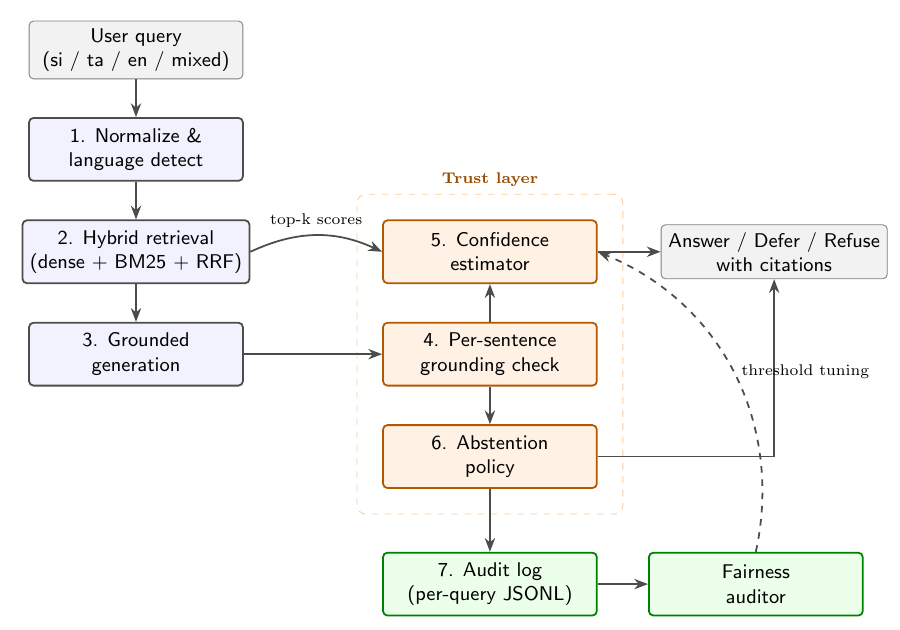
\includegraphics[width=\columnwidth]{figures/architecture.png}
  \caption{Pipeline. The trust layer (grounding, confidence, abstention, fairness audit) works on one audit record per decision, so a disparity surfaced by the auditor can be traced to retrieval scores or grounding support.}
  \Description{Flow diagram of seven stages: query normalisation, hybrid retrieval, grounded generation, grounding check, confidence, abstention policy, audit log feeding a fairness auditor.}
  \label{fig:pipeline}
\end{figure}
Figure~\ref{fig:pipeline} shows the pipeline. A script-based detector labels the query as si, ta, en, or \emph{mixed} (romanised code-switched text). Dense retrieval (multilingual-e5-base) and BM25~\cite{robertson1994bm25} are fused by reciprocal rank fusion~\cite{cormack2009rrf}, and the dense cosine of each hit is carried through fusion. The top-$k$ passages are passed to the generator with a prompt that asks it to answer only from the evidence, cite passages by number, reply in the query language, and emit \texttt{INSUFFICIENT\_EVIDENCE} when the evidence does not support an answer; that string is the generator's own abstention, which every compared system respects. It is detected anywhere in the reply, because small models often explain first; an earlier start-anchored detector scored such refusals as wrong answers and is corrected in every number here (\LRedetected{} cached 7B drafts). The pipeline is split into a \emph{draft} half (retrieve, generate) and a \emph{finalize} half (ground, score, decide, log), so the evaluation caches drafts once and replays every rule over the same drafts; all comparisons are exactly paired.

\paragraph{Grounding} For draft sentences $s_1,\dots,s_m$ and passages $P$, $g_i=\max_{p\in P}\mathrm{sup}(s_i,p)$, where $\mathrm{sup}$ is Jaccard overlap (offline) or the entailment probability of mDeBERTa-v3-xnli with $p$ as premise. Support is $G=\frac1m\sum_i g_i$; citation coverage $C$ is the fraction of sentences carrying a marker $[j]$, $j\le k$. Lexical overlap cannot match a Sinhala sentence to an English passage, so cross-script grounding needs the NLI checker.

\paragraph{Confidence} With $c_1,c_2$ the dense cosines of the top two hits and $\ell$ the language-match indicator (a retrieved chunk is in the query language or itself code-switched),
\begin{equation}
  s_{\mathrm{ret}}=\mathrm{clip}\tfrac{c_1-c_{\mathrm{lo}}}{c_{\mathrm{hi}}-c_{\mathrm{lo}}},\;
  s_{\mathrm{mar}}=\mathrm{clip}\,\kappa(c_1-c_2),\;
  s_{\mathrm{gr}}=G,\; s_{\mathrm{cit}}=C,\; s_{\mathrm{lang}}=\ell,
\end{equation}
with $c_{\mathrm{lo}},c_{\mathrm{hi}}$ the 5th/95th percentiles of $c_1$ and $\kappa$ the reciprocal 95th percentile of $c_1-c_2$ on the development split (7B: \LRetLo, \LRetHi, \LMarScale). The confidence is $\mathrm{conf}=\sum_x w_x s_x$ with default weights $0.20,0.20,0.40,0.10,0.10$. An earlier variant squashed the fused RRF scores, which lie in $(0,1/61]$, so the two retrieval signals added an almost constant offset and the score varied only with grounding and citation; it is kept as the ablation TriSafe-rrf. Optionally, conf is replaced by a Platt model over the five signals, or passed through isotonic or temperature scaling, all fitted on development labels.

\paragraph{Policy} Given conf $c$, support $G$, coverage $C$, the retrieved set, and the generator's abstention flag, the rule returns a decision and a machine-readable reason:
\begin{figure}[t]
\begin{small}
\begin{verbatim}
if no passages: REFUSE "no_evidence_retrieved"
if generator abstained: REFUSE "model_abstained"
if c < tau_ref: REFUSE "low_confidence"
if G < tau_g:   REFUSE "weak_grounding"
if c < tau_ans or C < tau_c:
                DEFER  "borderline_evidence"
else            ANSWER "ok"
\end{verbatim}
\end{small}
\caption{TriSafe-RAG abstention policy. Default thresholds $\tau_{\mathrm{ans}}{=}0.55$, $\tau_{\mathrm{ref}}{=}0.30$, $\tau_g{=}0.20$, $\tau_c{=}0.40$; the dev-tuned variant searches a grid over $(\tau_{\mathrm{ans}},\tau_{\mathrm{ref}},\tau_g)$ whose floor is $(0.30,0.10,0.10)$.}
\Description{Pseudo-code of the three-way abstention policy.}
\label{fig:policy}
\end{figure}
Per-language thresholds choose $\tau_{\mathrm{ans}}$ per language group on the development split; we evaluate this as a separate system, not a default.

\paragraph{Audit record and fairness audit} Every query writes one JSONL record: language, chunk ids and scores, the five signals, support, confidence, decision, reason, source paths, and hashes of draft and delivered text. The auditor reports per language group accuracy $A_g$ on answerable queries, answer rate $R_g$, TPR/FPR of the answer decision, and derives $\Delta A$, $\Delta R$, the Equalized Odds gap $\Delta EO=\max(\Delta\mathrm{TPR},\Delta\mathrm{FPR})$~\cite{hardt2016equality}, and cross-lingual consistency $\mathrm{CLC}=\max(0,1-\Delta A)$; groups with fewer than five queries are excluded from gaps. $\Delta R$ is printed beside $\Delta A$ because an accuracy gap also narrows when one language is simply answered less.

\paragraph{Metrics}\label{sec:metrics} \emph{Answered}: decision is \emph{answer} (defer and refuse are abstentions). \emph{Correct}: answerable query, answered, and a gold alias occurs in the delivered text (numbers matched as whole numbers, text as Unicode-normalised substrings); abstaining on an answerable query is an error. \emph{Accuracy} is mean correctness over answerable queries, \emph{selective accuracy} over answered answerable queries, \emph{unanswerable abstention} the share of unanswerable queries abstained on, and \emph{decision accuracy} the share of all queries either answerable-and-correct or unanswerable-and-abstained; it is the objective of every threshold search. \emph{Draft correctness} is whether the generator's draft matches the gold before any policy (for unanswerable queries: whether it abstained); ECE, AUROC, and the risk--coverage area are computed from confidence against draft correctness and are policy-independent, reported over all queries and over answered queries. \emph{Unsafe deliveries} $U$ are delivered wrong answers plus any answer to an unanswerable query; \emph{correct deliveries} $K$ match the gold; \emph{lost} is the number of correct drafts a rule withheld. If one unsafe delivery costs $c$ withheld correct answers, a rule's loss is $cU-K$ and its break-even against a reference is $c^*=(K_{\mathrm{ref}}-K)/(U_{\mathrm{ref}}-U)$: the rule is better for any $c>c^*$.

\section{The SL-PubServ-QA Benchmark}\label{sec:benchmark}
\paragraph{Corpus} \Lndocs{} documents (\Lnchunks{} chunks of at most 80 words) quoted from official publications of seven Sri Lankan agencies in three domains: civil documents (Immigration and Emigration, Registration of Persons, Motor Traffic and the eRL revenue-licence portal), public health (National Dengue Control Unit, Epidemiology Unit, Family Health Bureau), and disaster response (Disaster Management Centre, National Building Research Organisation, Department of Meteorology). Each document has a verbatim English section and Sinhala and Tamil summaries that preserve every number, drug name, and form code. One clearly labelled stale synthetic bulletin lists a past-season helpline (110) that contradicts the current hotline (117).

\paragraph{Items, queries, split} 62 items, 52 answerable and 10 unanswerable (out of scope, or supported only by the stale bulletin), each with an English question, Sinhala and Tamil translations, and for 22 items a romanised code-switched version (``passport normal service fee eka kiyada?''): \Lnq{} queries, 62 per single language and 22 code-switched. Gold answers are alias lists per item; two public-health items are false-premise prompts whose aliases express the correct negative. Because the same fact is asked in every language, per-language differences measure language effects, not question difficulty. Twelve item groups (\Lndev{} queries) form the development split, the remaining 50 (\Lntest{} queries: 50 per single language, 19 code-switched; 8 unanswerable per single language and 2 code-switched) the test split; a fact seen while tuning never appears in the test set in any language, and every threshold, weight, scale, and calibrator is chosen on the development split. Example items in all four query forms, typeset from the benchmark file, are in the supplement (S2).

%% auto-generated by scripts/native_review.py stats; do not edit
\newcommand{\ReviewStatus}{pending}
\paragraph{Provenance and limits} The English questions and gold aliases were written against the source text; the Sinhala and Tamil questions were produced by translating them and have not yet been independently verified by native speakers, which we flag as a limitation (Sec.~\ref{sec:discussion}). The corpus is small by design, so that every fact is traceable to a government URL; it does not measure retrieval at scale.


\section{Experimental Setup}\label{sec:setup}
\paragraph{Backends} The \emph{neural} backends use multilingual-e5-base, BM25, RRF with $\alpha{=}0.5$ and $k{=}4$, mDeBERTa-v3-base-xnli grounding, and one of two generators from one family~\cite{qwen2025qwen25}: Qwen2.5-7B-Instruct at 4-bit (Q4\_K\_M), the headline, and Qwen2.5-1.5B-Instruct at fp16, both served by llama.cpp/Ollama on one 8\,GB laptop GPU (temperature 0.2, nucleus 0.95, at most 128 new tokens). Each generator was run with \Lseeds{} sampling seeds; retrieval and the trust layer are deterministic given the draft. The \emph{offline} backend (hash embedder, an extractive generator that copies the best-overlapping evidence sentence and cannot fabricate, Jaccard grounding) is used for continuous integration and reported in the supplement (S6).

\paragraph{Systems} \emph{Ablations}: B1 \emph{vanilla} (retrieval and generation; the only abstention is the generator's own; its confidence, for calibration metrics, is $s_{\mathrm{ret}}$); B2 \emph{grounding only} (full confidence logged, no thresholds); B3 \emph{abstention only} (default policy on a confidence without grounding and citation, $w_{\mathrm{gr}}{=}w_{\mathrm{cit}}{=}0$). \emph{TriSafe-RAG} with default thresholds, dev-tuned thresholds, per-language thresholds, lexical grounding, the RRF signal, Platt-calibrated confidence, and without the language signal. \emph{Gate isolation}: the default policy with two of its three gates switched off. \emph{B1 + empty-reply filter}: B1 that refuses a draft containing nothing but citation markers (``[1] \#1''), motivated by the adjudication in Sec.~\ref{sec:cost}. \emph{External, training-free, same drafts}: E1 verbalized confidence~\cite{xiong2024verbalized} (a second call asks the model for a 0--100 confidence); E2 a gate on $s_{\mathrm{ret}}$, a proxy for CRAG's evaluator; E3 Platt, E4 isotonic, E5 temperature gates on the calibrated probability of draft correctness; E6 translate-then-retrieve (non-English queries translated to English by the same model, then the default policy; the translator is the small generator itself, so this is a floor for the approach); E7 self-consistency gate (three further drafts at temperature 0.7; the score is mean agreement of numbers or content words with the main draft; four generator calls per query). A \emph{show-the-passage} reference counts how often a gold alias occurs verbatim in the top-1 or top-4 passages.

\paragraph{Tuning and statistics} Every threshold is chosen by grid search on the development split to maximise decision accuracy, ties toward higher answer rate; development drafts of all seeds are pooled. Intervals are 95\% percentile intervals from a paired cluster bootstrap that resamples the 50 test items with all their language versions (2{,}000 draws, the same draws for every system, so difference intervals are paired)~\cite{koehn2004bootstrap}; significance against B1 uses two-sided sign-flip permutation tests with the sign flipped per item (10{,}000 permutations). Each query's outcome is averaged over seeds before resampling, so counts are means per seed and may be fractional; the seed noise is small (standard deviation of decision accuracy across seeds \LBoneDecSd{} for B1 and \LTunDecSd{} for TriSafe on the 7B) and is absorbed into the intervals. Section~\ref{sec:cv} repeats the tuning as a group 5-fold cross-fitting.

\section{Results}\label{sec:results}

\subsection{Main comparison}
\begin{table*}[t]
  \caption{Main results on the 169-query test split (neural7b backend). Ans.\ rate: fraction of queries answered. Acc.: accuracy on gold-answerable queries (abstention counts as an error). Sel.\ acc.: accuracy among answered answerable queries. Unans.\ abst.: fraction of unanswerable queries abstained on. Catch/Retain: share of wrong drafts on answerable queries that the policy abstained on, and share of correct drafts it delivered. ECE and AUROC are computed from the confidence score against draft correctness over all test queries (policy-independent). Brackets: 95\% paired bootstrap intervals over queries (2{,}000 resamples).}
  \label{tab:main-neural7b}
  \footnotesize
  \setlength{\tabcolsep}{3.5pt}
  \begin{tabular}{lcccccccc}
    \toprule
    System & Ans.\ rate & Acc.\ $\uparrow$ [95\% CI] & Sel.\ acc.\ $\uparrow$ & Unans.\ abst.\ $\uparrow$ & Catch/Retain & Abst.\ F1 $\uparrow$ & ECE $\downarrow$ [95\% CI] & AUROC $\uparrow$ \\
    \midrule
    B1 vanilla (LLM self-abstention only) & 0.69 & 0.527 [0.44, 0.60] & 0.649 & 0.96 & 0.39/0.99 & 0.641 & 0.242 [0.20, 0.34] & 0.541 \\
    B2 grounding only (no thresholds) & 0.69 & 0.527 [0.44, 0.60] & 0.649 & 0.96 & 0.39/0.99 & 0.641 & 0.311 [0.23, 0.37] & 0.438 \\
    B3 abstention only (w\_gr = 0) & 0.35 & 0.254 [0.18, 0.31] & 0.619 & 1.00 & 0.67/0.48 & 0.381 & 0.181 [0.14, 0.27] & 0.504 \\
    TriSafe-RAG (default thresholds) & 0.41 & 0.261 [0.17, 0.31] & 0.544 & 1.00 & 0.53/0.49 & 0.412 & 0.311 [0.23, 0.37] & 0.438 \\
    TriSafe-RAG with lexical (Jaccard) grounding & 0.02 & 0.014 [0.00, 0.04] & 0.750 & 1.00 & 0.99/0.03 & 0.270 & 0.232 [0.17, 0.31] & 0.539 \\
    TriSafe-RAG with raw RRF retrieval signal & 0.29 & 0.135 [0.06, 0.17] & 0.389 & 1.00 & 0.55/0.25 & 0.358 & 0.349 [0.26, 0.39] & 0.425 \\
    TriSafe-RAG (thresholds tuned on dev) & 0.48 & 0.343 [0.26, 0.41] & 0.600 & 1.00 & 0.51/0.64 & 0.459 & 0.311 [0.23, 0.37] & 0.438 \\
    TriSafe-RAG + per-language thresholds (dev) & 0.48 & 0.343 [0.26, 0.41] & 0.600 & 1.00 & 0.51/0.64 & 0.459 & 0.311 [0.23, 0.37] & 0.438 \\
    TriSafe-RAG with Platt-calibrated confidence & 0.49 & 0.345 [0.26, 0.41] & 0.602 & 1.00 & 0.51/0.65 & 0.460 & 0.083 [0.06, 0.20] & 0.550 \\
    \bottomrule
  \end{tabular}
\end{table*}

Table~\ref{tab:main-neural7b} reports the ablations and TriSafe variants on the 7B generator. B1 answers \LBoneAns{} of test queries (the rest are the generator's own abstentions) with accuracy \LBoneAcc{} and abstains on \LBoneUnans{} of unanswerable ones. Dev-tuned TriSafe-RAG answers \LTunAns{} with accuracy \LTunAcc{} (paired difference \LTunDeltaAcc, 95\% CI \LTunDeltaAccCI, permutation $p\LTunPcorrect$), abstains on every unanswerable query, catches \LTunCatch{} of the wrong drafts and retains \LTunRetain{} of the correct ones. Its selective accuracy, \LTunSel{} against \LBoneSel, is \emph{lower} than B1's: the policy withholds more correct drafts than wrong ones. Of its \LTunAbstN{} abstentions per seed, \LTunReasonmodelabstained{} are the generator's own refusals, which B1 also respects; the policy adds \LTunReasonborderlineevidence{} deferrals and \LTunReasonweakgrounding{} grounding refusals, and on seed 0 these withhold \LCaughtAll{} wrong and \LLostAll{} correct drafts (\LLosten{} of the correct ones English). B1's decision accuracy (\LBoneDec) is therefore higher than that of every TriSafe variant (\LTunDec{} dev-tuned, \LTPlattDec{} Platt-calibrated), and than the gates E1--E5, all of which the tuning returns identical to B1 (decision accuracy \LEoneDec): on the \Lndev-query development split the objective is maximised by never abstaining beyond the generator. The TriSafe grid cannot return that rule, because its floor ($\tau_{\mathrm{ans}}{=}0.30$, $\tau_g{=}0.10$) still refuses weakly grounded drafts, a safety requirement fixed before the run; the price of the requirement on this generator is the gap between \LTunDec{} and \LBoneDec, on the development split as well (\LTunDevDec{} against \LBoneDevDec). The search returns that floor in every configuration (Secs.~\ref{sec:fair} and~\ref{sec:cv}), and Platt scaling changes no decision, so the dev-tuned rule is in effect the grounding gate plus the citation gate. The full external-baseline table is in the supplement (S3).

\paragraph{Calibration} The confidence columns are policy-independent, and they go against our design: B1's retrieval similarity has ECE \LBoneEce{} and AUROC \LBoneAuroc; the five-signal sum has ECE \LTunEce{} and AUROC \LTunAuroc{} (ECE difference \LTunDeltaEce, CI \LTunDeltaEceCI). Over answered drafts only, which removes the generator's abstentions from the comparison, the ranking is the same (\LBoneEceAns{} against \LTunEceAns). The grounding-weight sweep (supplement S3) shows ECE rising monotonically with $w_{\mathrm{gr}}$: the cross-lingual NLI checker assigns high support to wrong Sinhala and Tamil drafts, so the signal with the largest weight is the least reliable across scripts. Platt scaling of the same signals repairs calibration (ECE \LTPlattEce, \LTPlattEceAns{} on answered drafts) without changing a decision. Lexical grounding gives answer rate \LLexAns, because Sinhala--English overlap is near zero, and the RRF signal answers \LRrfAns.

\subsection{Which gate does the work}\label{sec:gates}
\begin{table*}[t]
  \caption{Which gate does the work (neural7b backend, test split). ``B1 + empty-reply filter'' refuses replies that contain nothing but citation markers. Each ``only'' row keeps one gate of the policy in Fig.~\ref{fig:policy} at its default threshold and switches the other two off (a threshold of 0 never fires); all rows respect the generator's own abstention, as B1 does. Unsafe: delivered answers that were wrong or answered an unanswerable query. Lost: correct drafts the policy withheld. Break-even: the cost of one unsafe delivery, in withheld correct answers, above which the row beats B1 (Sec.~\ref{sec:cost}); ``--'' when the row removes no unsafe deliveries.}
  \label{tab:gates-neural7b}
  \footnotesize
  \setlength{\tabcolsep}{4pt}
  \begin{tabular}{lcccccccc}
    \toprule
    Policy & Ans.\ rate & Acc.\ $\uparrow$ & Sel.\ acc.\ $\uparrow$ & Unans.\ abst.\ $\uparrow$ & Decision acc.\ $\uparrow$ & Unsafe $\downarrow$ & Lost $\downarrow$ & Break-even [95\% CI] \\
    \midrule
    B1 vanilla & 0.69 & 0.510 & 0.635 & 0.96 & 0.580 & 43 & 1 & -- \\
    B1 + empty-reply filter & 0.51 & 0.510 & 0.859 & 0.96 & 0.580 & 13 & 1 & 0.0 [0.0, 0.0] \\
    confidence thresholds only & 0.53 & 0.350 & 0.562 & 1.00 & 0.450 & 39 & 24 & 5.8 [2.3, 25.0] \\
    grounding gate only & 0.62 & 0.462 & 0.629 & 1.00 & 0.544 & 39 & 8 & 1.8 [0.5, 9.0] \\
    citation gate only & 0.52 & 0.364 & 0.591 & 1.00 & 0.462 & 36 & 22 & 3.0 [1.4, 9.0] \\
    TriSafe-RAG (default) & 0.42 & 0.266 & 0.535 & 1.00 & 0.379 & 33 & 36 & 3.5 [1.9, 8.8] \\
    TriSafe-RAG (dev-tuned) & 0.50 & 0.350 & 0.595 & 1.00 & 0.450 & 34 & 24 & 2.6 [1.3, 6.8] \\
    TriSafe-RAG (dev-tuned) + empty-reply filter & 0.33 & 0.350 & 0.893 & 1.00 & 0.450 & 6 & 24 & 0.6 [0.3, 1.0] \\
    TriSafe-RAG, $w_{\mathrm{lang}}=0$ & 0.38 & 0.224 & 0.500 & 1.00 & 0.343 & 32 & 42 & 3.7 [2.1, 8.6] \\
    B3 abstention only & 0.36 & 0.259 & 0.607 & 1.00 & 0.373 & 24 & 37 & 1.9 [1.1, 3.4] \\
    \bottomrule
  \end{tabular}
\end{table*}

Table~\ref{tab:gates-neural7b} switches off two of the three gates at a time (counts are means per seed). B1 delivers \LBoneUnsafe{} unsafe answers; the confidence thresholds alone leave \LGateConfUnsafe{} (\LGateConfLost{} correct drafts lost), the grounding gate \LGateGrUnsafe{} (\LGateGrLost), the citation gate \LGateCitUnsafe{} (\LGateCitLost), the default policy \LDefUnsafe{} (\LDefLost), and the dev-tuned policy \LTunUnsafe{} (\LTunLost). No single gate removes more than a quarter of the unsafe deliveries; the grounding gate is the cheapest (break-even \LGateGrBreakEven), the confidence thresholds the most expensive (\LGateConfBreakEven). Dropping the language signal makes the rule stricter (\LNolangUnsafe{} unsafe, \LNolangLost{} lost) without a better trade.

The decisive row is the empty-reply filter. Adjudicating every answer B1 delivered on seed 0 (Sec.~\ref{sec:cost}) showed that \LAdjEmpty{} of \LAdjN{} consist of nothing but citation markers; a check that refuses such replies, with no threshold and no model, cuts unsafe deliveries from \LBoneUnsafe{} to \LBemptyUnsafe{} at a cost of \LBemptyLostVsBone{} correct answers relative to B1. The gates were designed for confident hallucinations; on this generator the dominant Sinhala and Tamil failure is a reply with no content, which passes the citation gate (it cites) and often the grounding gate, and which no confidence threshold targets.

\subsection{The cost of a wrong answer}\label{sec:cost}
\begin{table*}[t]
  \caption{Delivered answers on the 169-query test split (neural7b backend), expected counts over seeds with paired bootstrap intervals. Correct: delivered answers matching the gold. Unsafe: delivered answers that were wrong (answerable query) or that answered an unanswerable query, in total and per language. Lost: correct drafts the decision rule withheld. Break-even: the cost of one unsafe delivery, measured in withheld correct answers, at which the system's loss $c\cdot U-K$ equals B1's; the system is the better choice for any cost above it. E6 produces different drafts and is listed for completeness.}
  \label{tab:cost-neural7b}
  \footnotesize
  \setlength{\tabcolsep}{3.5pt}
  \begin{tabular}{lcccccccc}
    \toprule
    System & Correct $\uparrow$ [95\% CI] & Unsafe $\downarrow$ [95\% CI] & en & si & ta & mixed & Lost $\downarrow$ & Break-even vs.\ B1 [95\% CI] \\
    \midrule
    B1 vanilla & 75.3 [63.7, 87.3] & 41.7 [32, 51.3] & 2.7 & 19.3 & 18.3 & 1.3 & 0.7 & -- \\
    B1 + empty-reply filter & 75 [63, 86.7] & 15 [9.3, 20.7] & 0.7 & 7.7 & 6.3 & 0.3 & 1 & 0.0 [0.0, 0.0] \\
    TriSafe-RAG (default) & 37.3 [28.7, 46.7] & 31.3 [23.3, 40] & 0 & 14.7 & 16 & 0.7 & 38.7 & 3.7 [2.2, 7.2] \\
    TriSafe-RAG (dev-tuned) & 49 [39.7, 59.3] & 32.7 [24.3, 41.3] & 1 & 14.7 & 16.3 & 0.7 & 27 & 2.9 [1.6, 6.0] \\
    TriSafe-RAG (dev-tuned) + empty-reply filter & 48.7 [39.3, 59] & 8 [4.3, 12] & 0 & 3.3 & 4.3 & 0.3 & 27.3 & 0.8 [0.5, 1.2] \\
    TriSafe-RAG (per-language) & 49 [39.7, 59.3] & 32.7 [24.3, 41.3] & 1 & 14.7 & 16.3 & 0.7 & 27 & 2.9 [1.6, 6.0] \\
    TriSafe-RAG (Platt conf.) & 49.3 [40, 59.7] & 32.7 [24.3, 41.3] & 1 & 14.7 & 16.3 & 0.7 & 26.7 & 2.9 [1.6, 5.9] \\
    E1 verbalized confidence & 75.3 [63.7, 87.3] & 41.7 [32, 51.3] & 2.7 & 19.3 & 18.3 & 1.3 & 0.7 & -- \\
    E2 retrieval gate & 75.3 [63.7, 87.3] & 41.7 [32, 51.3] & 2.7 & 19.3 & 18.3 & 1.3 & 0.7 & -- \\
    E3 Platt gate & 75.3 [63.7, 87.3] & 41.7 [32, 51.3] & 2.7 & 19.3 & 18.3 & 1.3 & 0.7 & -- \\
    E4 isotonic gate & 75.3 [63.7, 87.3] & 41.7 [32, 51.3] & 2.7 & 19.3 & 18.3 & 1.3 & 0.7 & -- \\
    E5 temperature gate & 75.3 [63.7, 87.3] & 41.7 [32, 51.3] & 2.7 & 19.3 & 18.3 & 1.3 & 0.7 & -- \\
    E6 translate-then-retrieve & 32.7 [24.3, 42.7] & 0.7 [0, 1.7] & 0 & 0.3 & 0.3 & 0 & 51.3 & 1.0 [0.7, 1.6] \\
    E7 self-consistency gate & 75.3 [63.7, 87.3] & 41.7 [32, 51.3] & 2.7 & 19.3 & 18.3 & 1.3 & 0.7 & -- \\
    \bottomrule
  \end{tabular}
\end{table*}

Decision accuracy weighs a withheld correct answer and a delivered wrong one equally, which no public-service deployment does. Table~\ref{tab:cost-neural7b} reports the two separately with break-even costs against B1 and against the empty-reply filter. B1 delivers \LBoneCorrect{} correct and \LBoneUnsafe{} unsafe answers, almost all wrong answers in Sinhala and Tamil rather than answers to unanswerable questions (\LBoneUnsafeUnans). Dev-tuned TriSafe-RAG delivers \LTunCorrect{} correct and \LTunUnsafe{} unsafe (\LTunLost{} correct drafts withheld, \LBoneLost{} of which B1 also withholds), so its break-even is \LTunBreakEven{} (95\% CI \LTunBreakEvenCI). It is never the best of the ablations: B1 beats it below that cost, and B3, the retrieval-only abstention rule at default thresholds (\LBthreeUnsafe{} unsafe, \LBthreeCorrect{} correct, break-even \LBthreeBreakEven{} against B1), beats it above a cost of \LCrossTunBthree. The gates E1--E5 remove nothing and have no break-even.

\paragraph{Self-consistency} E7 tunes to a threshold of zero on the pooled development drafts and also removes nothing, although on seed 0 alone it was the cheapest rule: tuned on that seed its threshold was \LEsevenFixThr, removing \LEsevenFixRemovedSeedZero{} unsafe deliveries at \LEsevenFixLostSeedZero{} lost. With three seeds every positive threshold lowers development decision accuracy (\LEsevenDevDecZero{} at zero, \LEsevenDevDecFix{} at \LEsevenFixThr), and the protocol selects zero. At the seed-0 threshold it would remove \LEsevenFixRemoved{} unsafe deliveries per seed at \LEsevenFixLost{} lost on the test split (break-even \LEsevenFixBreakEven): a cheap gate whose tuning \Lndev{} development queries cannot fix. We report it as the protocol tunes it.

\paragraph{Empty replies} The adjudication (one seed, every delivered test answer; the labels were produced by an AI assistant and reviewed by the author) classified \LAdjStrictCorrect{} of \LAdjNAns{} delivered answerable answers as correct, \LAdjPartial{} as partial, and the rest wrong; alias matching agrees with it on \LAdjAgreeStrict\% (\LAdjFP{} false positives, \LAdjFN{} false negatives), and \LAdjWrongLang{} answers are in Chinese. Its main finding is that \LAdjEmpty{} delivered answers (\LAdjEmptysi{} Sinhala, \LAdjEmptyta{} Tamil) are citation-only. Because the filter was found on test answers it is a post-hoc rule, so we check it where it was not found: on the development split it cuts B1's unsafe deliveries from \LBoneDevUnsafe{} to \LBemptyDevUnsafe{} with correct deliveries unchanged (\LBoneDevCorrect), and on the 1.5B generator, which rarely produces such replies, from \NBoneDevUnsafe{} to \NBemptyDevUnsafe{} (development) and \NBoneUnsafe{} to \NBemptyUnsafe{} (test). We also regenerated the \LProbeN{} seed-0 citation-only replies with the same model and passages: with the benchmark prompt \LProbeBaseEmpty{} are empty again; raising the cap from 128 to 512 tokens leaves \LProbeTokensEmpty; adding one sentence to the prompt that forbids a citation-only reply leaves \LProbeInstructEmpty, and the model then answers \LProbeInstructCorrect{} of the \LProbeN{} correctly and \LProbeInstructWrong{} wrongly. The replies are therefore a prompt-sensitive generator behaviour, not a token cap. A prompt fix would recover about half of these queries as correct answers, which the filter cannot; we did not rerun the benchmark with the changed prompt, so this is a limitation of B1's prompt that the reader should weigh, and B1 with the filter is the fair vanilla baseline for the prompt as run.

\paragraph{Ranking} Adding dev-tuned TriSafe-RAG to the filter leaves \LTemptyUnsafe{} unsafe deliveries at \LTemptyCorrect{} correct: a break-even of \LTemptyBreakEven{} against B1, but \LTemptyBreakEvenEmpty{} (95\% CI \LTemptyBreakEvenEmptyCI) against the filter alone, which is the relevant comparator. Translate-then-retrieve, which we had listed as a weak baseline, has the fewest unsafe deliveries in the table (\LEsixUnsafe, with \LEsixCorrect{} correct); its break-even against the filter is \LEsixBreakEvenEmpty{} (\LEsixBreakEvenEmptyCI) and against TriSafe plus filter \LCrossEsixTempty. The ranking a deployment should take from the table is therefore: refuse empty replies at any cost; above a cost of about \LEsixBreakEvenEmpty{} withheld correct answers per wrong one, translate the query before retrieval; and the reference rule, with or without the filter, is nowhere the lowest-loss choice on this generator.

\paragraph{Show the passage} A gold alias occurs in the top-ranked passage for \LShowTopone{} of the \LShowN{} answerable test queries (\LShowToponePct\%) and in the top four for \LShowTopk{} (\LShowTopkPct\%), against \LBoneCorrect{} correct generator deliveries: the evidence is on the page far more often than the generator manages to say it. The passages are English, so for Sinhala and Tamil users this is a reference point, not a system.

\subsection{Cross-lingual fairness}\label{sec:fair}
\begin{table*}[t]
  \caption{Per-language results on the test split (neural7b backend). Each language cell is accuracy on answerable queries / answer rate, so a narrowing accuracy gap can be read against coverage. $\Delta A$: max--min accuracy gap over the three single-language groups and the code-switched group with at least five test queries; $\Delta R$: the same gap for answer rate; $\Delta EO$: max of the TPR and FPR gaps on the answer/abstain decision; CLC $= 1-\Delta A$. Test queries per language: en: 50 (8 unans.), si: 50 (8 unans.), ta: 50 (8 unans.), mixed: 19 (2 unans.).}
  \label{tab:fair-neural7b}
  \footnotesize
  \setlength{\tabcolsep}{3.5pt}
  \begin{tabular}{lcccccccc}
    \toprule
    System & en & si & ta & mixed & $\Delta A \downarrow$ [95\% CI] & $\Delta R \downarrow$ & $\Delta EO \downarrow$ & CLC $\uparrow$ \\
    \midrule
    B1 vanilla (LLM self-abstention only) & 0.93/0.84 & 0.19/0.56 & 0.31/0.64 & 0.76/0.74 & 0.74 [0.61, 0.88] & 0.28 & 0.31 & 0.26 \\
    B3 abstention only (w\_gr = 0) & 0.52/0.46 & 0.10/0.26 & 0.14/0.40 & 0.29/0.26 & 0.43 [0.28, 0.61] & 0.20 & 0.25 & 0.57 \\
    TriSafe-RAG (default thresholds) & 0.48/0.40 & 0.14/0.42 & 0.17/0.50 & 0.29/0.26 & 0.33 [0.20, 0.54] & 0.24 & 0.30 & 0.67 \\
    TriSafe-RAG (thresholds tuned on dev) & 0.67/0.58 & 0.14/0.42 & 0.17/0.50 & 0.53/0.47 & 0.52 [0.39, 0.72] & 0.16 & 0.19 & 0.48 \\
    TriSafe-RAG + per-language thresholds (dev) & 0.67/0.58 & 0.14/0.42 & 0.17/0.50 & 0.53/0.47 & 0.52 [0.39, 0.72] & 0.16 & 0.19 & 0.48 \\
    \bottomrule
  \end{tabular}
\end{table*}

Table~\ref{tab:fair-neural7b} reports accuracy and answer rate per language. B1's accuracy gap over the single-language groups is \LBoneGap{} and its Equalized Odds gap \LBoneEO; dev-tuned TriSafe's are \LTunGap{} and \LTunEO{} (paired $\Delta A$ difference \LTunDeltaGap, CI \LTunDeltaGapCI). The narrower gap is produced by levelling down: English accuracy falls from \LBoneAccen{} to \LTunAccen{} while Sinhala moves from \LBoneAccsi{} to \LTunAccsi, so a smaller $\Delta A$ is not evidence of better service to Sinhala or Tamil users. The generator abstains on \LModelAbstsi{} of Sinhala and \LModelAbstta{} of Tamil test queries before any policy (\LModelAbsten{} in English), and its draft accuracy is \LDraftAccen{} (en), \LDraftAccsi{} (si), \LDraftAccta{} (ta); yet the top-4 passages contain a gold alias for \LRetHitsi{} of Sinhala and \LRetHitta{} of Tamil queries. The failure is cross-lingual reading, not retrieval, and a Sinhala-capable generator is the first thing a deployment would change. The policy leaves \LTunUnsafesi{} of B1's \LBoneUnsafesi{} unsafe Sinhala deliveries in place, because an empty reply cites a passage and the NLI checker often scores it as supported. Per-language thresholds tuned on about ten development queries per language all return the global floor (0.30) and change no test decision; we show this variant as proof that the audit can be turned into enforcement, not as a default. With 8 unanswerable test queries per language and 2 code-switched, the per-language FPR behind $\Delta EO$ rests on eight decisions per group, and the code-switched group has 19 test queries; where intervals overlap we draw no conclusion.

\subsection{Generator scale}\label{sec:scale}
The 1.5B generator (full tables in the supplement, S5) abstains on \NModelAbstsi{} of Sinhala queries against \LModelAbstsi{} for the 7B and has decision accuracy \NBoneDec{} (B1) against \NTunDec{} (dev-tuned TriSafe), so the regime of Sec.~\ref{sec:results}, a generator that already abstains and a policy that then withholds more correct answers than wrong ones, holds at both sizes (break-even \NTunBreakEven, 95\% CI \NTunBreakEvenCI). Two findings do not transfer. Citation-only replies are a 7B behaviour (one to three per seed at 1.5B), so the filter does nothing there; and the calibration comparison reverses (five-signal ECE \NTunEce{} against retrieval \NBoneEce{} at 1.5B), so the negative calibration result is a property of this generator and checker pair, not of the signal set. The 4-bit quantisation of the 7B model is a confound in this comparison; it does not fit the GPU at higher precision.

\subsection{Robustness of the tuning}\label{sec:cv}
A group \LCvFolds-fold cross-fitting over all \Lnq{} queries (supplement S7) tunes the TriSafe thresholds and the E1 and E7 gates on four folds and applies them to the fifth. Out-of-fold decision accuracy is \LCvBoneDec{} for B1 and \LCvTunDec{} for TriSafe (paired difference \LCvTunDeltaDec, 95\% CI \LCvTunDeltaDecCI), with \LCvBoneUnsafe{} against \LCvTunUnsafe{} unsafe deliveries and a break-even of \LCvTunBreakEven. Every fold returns $\tau_{\mathrm{ans}}=\LCvTauAns$, the floor of the grid: the development/test result is not an artefact of one split, and the confidence thresholds are inactive in the tuned rule under any split.

\section{Discussion and Threats to Validity}\label{sec:discussion}
\paragraph{Evidence present but wrong} Refusing when evidence is missing is the easy case. The grounding check marks a sentence copied from the stale bulletin as supported, so nothing in the trust layer distinguishes a stale passage from a current one; on the stale-bulletin probes (supplement S4) it is the generator's own refusal that produces the safe outcome, and the source path in the audit record is what lets an operator retire such passages.

\paragraph{When the generator already abstains} The offline generator never abstains, and the policy supplies the missing caution (unanswerable abstention \OBoneUnans{} to \OTunUnans, supplement S6). Qwen2.5-7B abstains by itself on a third to a half of Sinhala and Tamil queries, and when it does not it often returns a citation without content; the policy's extra abstentions then fall largely on correct English drafts while the content-free replies pass. Whether a post-hoc abstention layer helps is a property of the generator it wraps, per language, and the audit record provides the abstention, draft-accuracy, and empty-reply rates needed to decide that before deployment.

\paragraph{Validity} The corpus is small and retrieval is easy at this scale; both generators are weaker in Sinhala and Tamil than hosted models, and we ran no hosted model. Alias matching rewards a correct value anywhere in the text and penalises unlisted spellings; the adjudication bounds its error at \LAdjFP{} false positives in \LAdjN{} answers, and an LLM judge would be a useful complement. The translations were machine-drafted and reviewed query by query by one author who is a native speaker of both languages, with no query changed; this is one reviewer, not an inter-annotator study, and the Sinhala and Tamil summaries inside the corpus documents have not been reviewed (a review sheet is released). Residual translation error would lower non-English accuracy for every rule equally. Fairness is audited, not guaranteed: with per-language thresholds the rule can be adjusted, but the choice is a policy decision resting on a small development set. The confidence is a fixed weighted sum, kept so that every reason in the audit log traces to a signal; the development objective is flat across the grounding-weight sweep and gives no guidance for choosing the weights.

\section{Conclusion}\label{sec:conclusion}
SL-PubServ-QA, the audit record, and the cost analysis let any answer/defer/refuse rule be measured per language and priced by what a wrong answer must cost for the rule to pay off. Measured this way, our reference rule does not win: dev-tuned TriSafe-RAG cuts unsafe deliveries per seed from \LBoneUnsafe{} to \LTunUnsafe{} but delivers \LTunLostVsBone{} fewer correct answers, pays off against the vanilla pipeline only above a cost of \LTunBreakEven, is beaten by a retrieval-only rule above \LCrossTunBthree, and its five-signal confidence is not better calibrated than retrieval similarity. A content filter for citation-only replies, found by reading the delivered answers and confirmed on the development split and a second generator, removes most unsafe deliveries at almost no cost; translating the query wins above a cost of about \LEsixBreakEvenEmpty; and a self-consistency gate that looked free on one seed tunes to inaction on three. The lesson is that an abstention layer has to be designed against the measured failure modes of its generator, per language, and that the audit record and an adjudication of delivered answers are what make those failure modes visible before deployment. Limits: a small corpus, open-weight generators of 1.5B and 7B parameters with the 7B at 4-bit, three seeds, one native-speaker reviewer, and an audit rather than a guarantee.

\paragraph{Reproducibility} Code, the benchmark with its review sheets, the per-seed draft caches of every backend, per-system per-query records, the adjudication labels, and the scripts that regenerate every macro, table, and figure are provided as anonymised supplementary material and will be released publicly.

\section*{GenAI Usage Disclosure}
Generative AI was used in three ways. (a)~\emph{As systems under study:} Qwen2.5-1.5B-Instruct and Qwen2.5-7B-Instruct served as generator, translator, self-consistency sampler, and verbalized-confidence source; multilingual-e5 and mDeBERTa-v3 as retriever and grounding checker (Sec.~\ref{sec:setup}). (b)~\emph{In building the artefacts:} an AI assistant (Claude, Anthropic) implemented and tested evaluation code, drafted the Sinhala and Tamil translations of the benchmark questions and the alias lists, produced the adjudication labels of Sec.~\ref{sec:cost}, and generated tables and figures from the recorded results. (c)~\emph{In preparing the manuscript:} the same assistant drafted and copy-edited text and checked cross-references. The research questions, system design, protocol, and all claims are the author's own; the author reviewed every statement and every adjudication label, and every machine-drafted Sinhala, Tamil, and code-switched query was reviewed by the author, a native speaker of Sinhala and Tamil (Sec.~\ref{sec:benchmark}).

\bibliographystyle{ACM-Reference-Format}
\bibliography{refs}
